\documentclass{beamer}
\usetheme[titlepagelogo=img/bicocca,% Logo for the first page
		  language=italian,
		  assistantsupervisor=true,
		  secondlogo=true,
		  bullet=triangle,
		  color=red,
		  pageofpages=di,
		  shadow=false
         ]{TorinoTh}
         
\usepackage[beamer,customcolors]{hf-tikz}
\hfsetfillcolor{alerted text.fg!10}
\hfsetbordercolor{alerted text.fg}

\titlepagesecondlogo{img/ira.jpg}
\author{Federica Di Lauro}
\rel{Prof. Domenico G. Sorrenti}
\assistantsupervisor{Dott. Simone Fontana}
\title{Sistema di controllo per base robotica outdoor}
\ateneo{Università degli studi di Milano-Bicocca}
\date{24 luglio 2020}

\begin{document}

\titlepageframe % Specific command 

\begin{tframe}{Obiettivi}

\begin{columns}
\begin{column}{0.45\textwidth}
Cose cose cose cose:
\begin{itemize}
    \item Ricerca e installazione hardware mancante
    \item Progettazione e sviluppo sistema di controllo
    \item Integrazione con il framework ROS
\end{itemize}

\end{column}

\begin{column}{0.45\textwidth}
\begin{center}
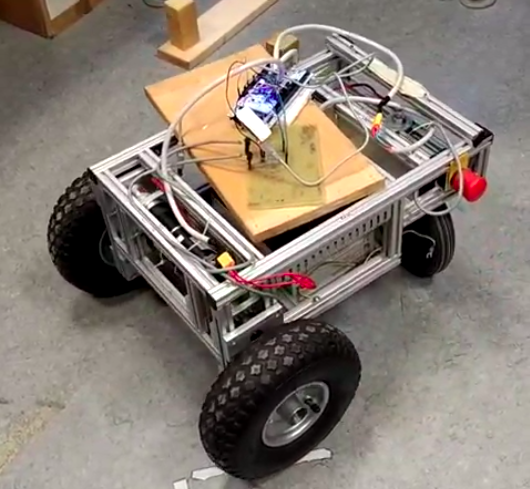
\includegraphics[width=0.9\columnwidth]{img/otto2.png}
\end{center}
\end{column}
\end{columns}
\end{tframe}

\begin{tframe}{Infrastruttura hardware}
\begin{center}
    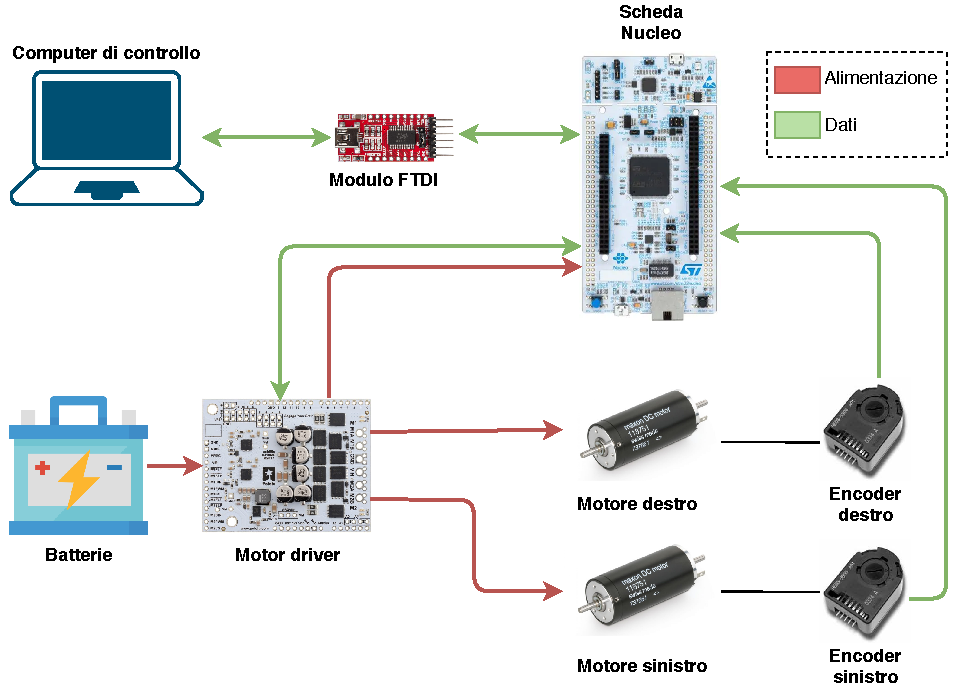
\includegraphics[width=0.8\textwidth]{img/infrastruttura.pdf}
\end{center}
\end{tframe}

\begin{tframe}{Progettazione sistema}
\begin{itemize}
\item Lato microcontrollore:
\begin{itemize}
    \item Lettura ed elaborazione dati degli encoder
    \item Controllo dei motori tramite un sistema in retroazione
    \item Comunicazione bidirezionale con un computer di controllo
\end{itemize}
\item Lato computer:
 \begin{itemize}
    \item Comunicazione con il microcontrollore
    \item Calcolo odometria
    \item Integrazione con ROS
\end{itemize}
\end{itemize}

\end{tframe}

\begin{tframe}{Sviluppo microcontrollore: Encoder}

\end{tframe}

\begin{tframe}{Sviluppo microcontrollore: Motori e PID}

\end{tframe}

\begin{tframe}{Sviluppo microcontrollore: Comunicazione}

\end{tframe}

\begin{tframe}{Sviluppo computer: Nodo ROS}

\end{tframe}

\begin{tframe}{Testing}

\end{tframe}

\begin{tframe}{Conclusioni}

\end{tframe}

\begin{tframe}{Grazie per l'attenzione}

\end{tframe}

\end{document}